%\documentclass[10pt,handout]{beamer}
\documentclass[11pt]{beamer}\usepackage[]{graphicx}\usepackage[]{color}
%% maxwidth is the original width if it is less than linewidth
%% otherwise use linewidth (to make sure the graphics do not exceed the margin)
\makeatletter
\def\maxwidth{ %
  \ifdim\Gin@nat@width>\linewidth
    \linewidth
  \else
    \Gin@nat@width
  \fi
}
\makeatother

\definecolor{fgcolor}{rgb}{0.196, 0.196, 0.196}
\newcommand{\hlnum}[1]{\textcolor[rgb]{0.063,0.58,0.627}{#1}}%
\newcommand{\hlstr}[1]{\textcolor[rgb]{0.063,0.58,0.627}{#1}}%
\newcommand{\hlcom}[1]{\textcolor[rgb]{0.588,0.588,0.588}{#1}}%
\newcommand{\hlopt}[1]{\textcolor[rgb]{0.196,0.196,0.196}{#1}}%
\newcommand{\hlstd}[1]{\textcolor[rgb]{0.196,0.196,0.196}{#1}}%
\newcommand{\hlkwa}[1]{\textcolor[rgb]{0.231,0.416,0.784}{#1}}%
\newcommand{\hlkwb}[1]{\textcolor[rgb]{0.627,0,0.314}{#1}}%
\newcommand{\hlkwc}[1]{\textcolor[rgb]{0,0.631,0.314}{#1}}%
\newcommand{\hlkwd}[1]{\textcolor[rgb]{0.78,0.227,0.412}{#1}}%

\usepackage{framed}
\makeatletter
\newenvironment{kframe}{%
 \def\at@end@of@kframe{}%
 \ifinner\ifhmode%
  \def\at@end@of@kframe{\end{minipage}}%
  \begin{minipage}{\columnwidth}%
 \fi\fi%
 \def\FrameCommand##1{\hskip\@totalleftmargin \hskip-\fboxsep
 \colorbox{shadecolor}{##1}\hskip-\fboxsep
     % There is no \\@totalrightmargin, so:
     \hskip-\linewidth \hskip-\@totalleftmargin \hskip\columnwidth}%
 \MakeFramed {\advance\hsize-\width
   \@totalleftmargin\z@ \linewidth\hsize
   \@setminipage}}%
 {\par\unskip\endMakeFramed%
 \at@end@of@kframe}
\makeatother

\definecolor{shadecolor}{rgb}{.97, .97, .97}
\definecolor{messagecolor}{rgb}{0, 0, 0}
\definecolor{warningcolor}{rgb}{1, 0, 1}
\definecolor{errorcolor}{rgb}{1, 0, 0}
\newenvironment{knitrout}{}{} % an empty environment to be redefined in TeX

\usepackage{alltt}
%\documentclass[11pt, handout]{beamer}
%\usepackage{handoutWithNotes}
%\usepackage{pgfpages}
\usepackage{etex} % helps fix \newdimen error which is cause when ctable is loaded with other packages
\usepackage{comment}
\usepackage{ctable}
\usepackage{amsmath,amsthm,amssymb}
\newtheorem{rcode}{R Code}[section]
\usepackage{url}

%\usepackage[usenames]{xcolor}
\usepackage{color, colortbl}
\usepackage{tikz}
\usepackage[utf8]{inputenc}
\usepackage[T1]{fontenc}
\usepackage{ae}
%\usepackage{aeguill}

\usetikzlibrary{shapes.geometric, arrows,shapes.symbols,decorations.pathreplacing}
\tikzstyle{startstop} = [rectangle, rounded corners, minimum width=3cm, minimum height=1cm, draw=black, fill=pinkish,text width=3.5cm]
\tikzstyle{startstop2} = [rectangle, rounded corners, minimum width=3cm, minimum height=1cm, draw=black, fill=background,text width=2.5cm]
\tikzstyle{startstop3} = [rectangle, rounded corners, minimum width=3cm, minimum height=1cm, draw=black, fill=beige,text width=3.0cm]
\tikzstyle{io} = [trapezium, trapezium left angle=70, trapezium right angle=110, minimum width=2cm, minimum height=1cm, text centered, draw=black, fill=blue!30,text width=1.5cm]
\tikzstyle{process} = [rectangle, minimum width=1cm, minimum height=1cm, text centered, draw=black, fill=orange!30,text width=2cm]
\tikzstyle{decision} = [diamond, minimum width=2cm, minimum height=1cm, text centered, draw=black, fill=green!30]
\tikzstyle{arrow} = [thick,->,>=stealth]
\tikzstyle{both} = [thick,<->,>=stealth, red]

\tikzset{myshade/.style={minimum size=.4cm,shading=radial,inner color=white,outer color={#1!90!gray}}}
\newcommand\mycirc[1][]{\tikz\node[circle,myshade=#1]{};}
\newcommand\myrect[1][]{\tikz\node[rectangle,myshade=#1]{};}
\newcommand\mystar[1][]{\tikz\node[star,star points=15,star point height=2pt,myshade=#1]{};}
\newcommand\mydiamond[1][]{\tikz\node[diamond,myshade=#1]{};}
\newcommand\myellipse[1][]{\tikz\node[ellipse,myshade=#1]{};}
\newcommand\mykite[1][]{\tikz\node[kite,myshade=#1]{};}
\newcommand\mydart[1][]{\tikz\node[dart,myshade=#1]{};}
\newcommand\mycloud[1][]{\tikz\node[cloud,myshade=#1]{};}

%\usepackage{subcaption}
\usepackage{subfig}
%\usepackage{caption}

\mode<presentation>
\usetheme{Hannover}
\usecolortheme{rose}
\setbeamertemplate{navigation symbols}{}
\setbeamertemplate{footline}[frame number]
\setbeamertemplate{caption}[numbered]
\setbeamertemplate{frametitle}[default][left]

\usepackage[]{hyperref}
\hypersetup{
    unicode=false,          
    pdftoolbar=true,        
    pdfmenubar=true,        
    pdffitwindow=false,     % window fit to page when opened
    pdfstartview={FitH},    % fits the width of the page to the window
    pdftitle={atelier R GERAD},    % title
    pdfauthor={Sahir Rai Bhatnagar},     % author
    pdfsubject={Subject},   % subject of the document
    pdfcreator={Sahir Rai Bhatnagar},   % creator of the document
    pdfproducer={Sahir Rai Bhatnagar}, % producer of the document
    pdfkeywords={}, % list of keywords
    pdfnewwindow=true,      % links in new window
    colorlinks=true,       % false: boxed links; true: colored links
    linkcolor=red,          % color of internal links (change box color with linkbordercolor)
    citecolor=blue,        % color of links to bibliography
    filecolor=black,      % color of file links
    urlcolor=cyan           % color of external links
}

%\RequirePackage{color}

% define a bunch of colors
\definecolor{gray}{RGB}{110,110,110}
\definecolor{darkgray}{RGB}{100,100,100}
\definecolor{lightgray}{RGB}{200,200,200}
\definecolor{turquoise}{RGB}{81,193,188}
\definecolor{tomato}{RGB}{255,136,136}
\definecolor{mandarina}{RGB}{229,169,25}
\definecolor{foreground}{RGB}{81,141,193}
\definecolor{background}{RGB}{246,244,240}
\definecolor{highlight}{RGB}{229,169,25}
\definecolor{lowlight}{RGB}{200,200,200}
\definecolor{beige}{RGB}{255,255,240}
\definecolor{pinkish}{RGB}{255,223,247}
%\definecolor{aliceblue}{rgb}{0.94, 0.97, 1.0}
%\definecolor{antiflashwhite}{rgb}{0.95, 0.95, 0.96}

% some convenient commands
\newcommand{\code}[1]{\texttt{#1}}
\newcommand{\high}[1]{\textcolor{highlight}{#1}}
\newcommand{\low}[1]{\textcolor{lowlight}{#1}}
\newcommand{\highcode}[1]{\textcolor{highlight}{\texttt{#1}}}

\setbeamercolor{block body}{bg=beige}

%\setbeamercovered{highly dynamic}

\newcounter{saveenumi}
\newcommand{\seti}{\setcounter{saveenumi}{\value{enumi}}}
\newcommand{\conti}{\setcounter{enumi}{\value{saveenumi}}}


%\setbeamercolor{subtitle}{fg=turquoise}

%\pgfpagesuselayout{4 on 1}[a4paper, landscape, border shrink=5mm]
%\pgfpagesuselayout{2 on 1 with notes landscape}[a4paper, border shrink=5mm]
\IfFileExists{upquote.sty}{\usepackage{upquote}}{}
\begin{document}





\title[Atelier sur le logiciel R]{Atelier sur le logiciel R}
\subtitle{Un introduction \`{a} la programmation en R}

\author[]{Sahir Rai Bhatnagar%
\thanks{\href{https://github.com/sahirbhatnagar/atelier-R-GERAD}{https://github.com/sahirbhatnagar/atelier-R-GERAD}%
}}

\date{29 juillet 2015}

%\makebeamertitle

\maketitle

\begin{frame}{Remerciements}
% \hspace*{-1.9cm}\parbox[t]{\textwidth}
%\frametitle{Acknowledgements}
\begin{columns}[c] % The "c" option specifies centered vertical alignment while the "t" option is used for top vertical alignment

\column{.45\textwidth} % Left column and width

\begin{itemize}
%\scriptsize
\item John Chambers
\item Ross Ihaka et Robert Gentleman
\item Greg Voisin
\item Dr. Vahid Partovi Nia
\item Toi
\end{itemize}

\column{.45\textwidth} % Right column and width
\begin{figure}
\includegraphics[width=0.6\columnwidth]{gerad.png}\\[2mm]
\includegraphics[width=0.6\columnwidth]{udem.png}\\[5mm]
\includegraphics[width=0.6\columnwidth]{hec.png}
%\includegraphics[width=0.7\columnwidth]{Logo-LUDMER.jpg}
\end{figure}

\end{columns}
\end{frame}


\begin{frame}{Avis \#1}
\begin{itemize}
\item Ce\c{c}i est un \textbf{introduction} au langage R
\pause \item On va faire beaucoup d'exercises
\pause \item N'h\'{e}sitez pas \`{a} posez des questions
\end{itemize}
\end{frame}

\begin{frame}{Avis \#2}
\begin{figure}
\includegraphics[width=1.0\columnwidth]{rstudio.png}\\[5mm]
\includegraphics[width=0.2\columnwidth]{rlogo.png}\\[5mm]
%\includegraphics[width=0.2\columnwidth]{LaTeX_logo.png}
\end{figure}

\textit{Je n'ai aucune relation commerciale avec ces logiciels}

\end{frame}

\begin{frame}{Avis \#3}

\begin{itemize}
\item Le mat\'{e}riel pour cet atelier est bas\'{e} sur plusieurs ressources
\item Voir ce lien pour une liste compl\`{e}te de r\'{e}f\'{e}rences: \href{https://github.com/sahirbhatnagar/atelier-R-GERAD}{https://github.com/sahirbhatnagar/atelier-R-GERAD}
\item Je vous sugg\`{e}re les livre de Vincent Goulet et Hadley Wickham
\end{itemize}

\begin{columns}[c] % The "c" option specifies centered vertical alignment while the "t" option is used for top vertical alignment
\column{.45\textwidth} % Left column and width
\begin{figure}
\includegraphics[width=0.8\columnwidth]{goulet.png}
\end{figure}

\column{.45\textwidth} % Right column and width
\begin{figure}
\includegraphics[width=0.6\columnwidth]{had.jpg}
\end{figure}
\end{columns}

\end{frame}


\begin{frame}[plain]{C'est parti}
\hspace*{-1.5cm}\parbox[t]{\textwidth}{
\begin{center}
\includegraphics[scale=0.51]{introR.jpg}
\end{center}
}
\end{frame}


\setbeamercolor{normal text}{fg=black,bg=background}
\begin{frame}[plain]
\hspace*{-1.0cm}\parbox[t]{\textwidth}{
\begin{block}{Après cet atelier vous devrez \^{e}tres capables de}
\begin{itemize}
\item Comprendre, créer et modifier les 4 objets de bases en R (\code{vector, data.frame, matrix, list}) 
\item Utiliser des fonctions de bases
\item Importé un jeux de donnés à partir d'un fichier externe
\item Créer un graphique 
\end{itemize}
\end{block}
}
\end{frame}


\section{1.Pr\'{e}sentation du langage R}

\setbeamercolor{normal text}{fg=gray,bg=black}
\begin{frame}[plain]
\hspace*{-1.0cm}\parbox[t]{\textwidth}{
 \begin{center}
  \Huge{\textcolor{white}{1. Pr\'{e}sentation du langage R}}
 \end{center}
 }
\end{frame}


\setbeamercolor{normal text}{fg=black,bg=background}
\begin{frame}[plain]
\hspace*{-1.0cm}\parbox[t]{\textwidth}{
\begin{block}{Objectifs du chapitre}
\begin{enumerate}
\item Comprendre les avantages d'apprendre R
\item Conna\^{\i}tre la provenance du R et ses charact\'{e}ristiques
\item D\'{e}marrer une session R et ex\'{e}cuter des commandes simple
\item Cr\'{e}er, modifier et sauvegarder ses propres fichiers de \mbox{script R}
\end{enumerate}
\end{block}
}
\end{frame}



\setbeamercolor{normal text}{fg=gray,bg=white}
\subsection{Pourquoi vous \^{e}tes l\`{a}?}

\begin{frame}
 \begin{center}
  \Huge{\textcolor{red}{Pourquoi vous \^{e}tes l\`{a}?}}
 \end{center}
\end{frame}


\begin{frame}{Le langage R gagne en popularit\'{e}}

\vspace{0.1in}

\begin{center}
\includegraphics[scale=0.40]{rankings.png}
\end{center}

\vspace{0.2in}

Les meilleurs langage de programmation en 2015 selon \href{http://spectrum.ieee.org/computing/software/the-2015-top-ten-programming-languages}{\mbox{IEEE Spectrum}} \\
\end{frame}


\begin{frame}{Plus de 100,000 questions pos\'{e}s dans les forums}

\includegraphics[scale=0.40]{stack.png}
\newline
\vspace{0.1in}
%\footenotesize{source: http://r4stats.com/articles/popularity/}
\end{frame}




\begin{frame}{Nombres d'emplois}

\begin{center}
\includegraphics[scale=0.47]{jobs.png}
\end{center}

\vspace{0.05in}

r\'{e}f\'{e}rence: \href{http://r4stats.com/articles/popularity/}{http://r4stats.com/articles/popularity/}\\

\end{frame}



\begin{frame}{Utilis\'{e} dans plusieurs domaines}

\begin{center}
\includegraphics[scale=0.31]{citeR.jpg}
\end{center}

\vspace{0.05in}

Publi\'{e} dans \href{http://www.nature.com/news/programming-tools-adventures-with-r-1.16609}{\textit{Nature}}
\end{frame}


\begin{frame}{Analyser vos données}
\begin{itemize}
  \setlength\itemsep{2em}
\item \'{E}norme resources d'outils statistiques
\item Représenter graphiquement des jeux de données multivariables
\item Intégrer votre code R avec des sites internet
\item Assurer la reproductivité de vos analyses
\end{itemize}
\end{frame}



\subsection{Bref historique}

\begin{frame}
 \begin{center}
  \Huge{\textcolor{red}{Bref historique}}
 \end{center}
\end{frame}


\begin{frame}{\`{A} l'origine de R fut le S par John M. Chambers}
\begin{center}
\begin{figure}
\includegraphics[scale=0.10]{john.jpg}
\caption{S, un langage pour programmer avec des donn\'{e}es, developp\'{e} chez Bell Laboratories dans les ann\'{e}es 1970 par une \'{e}quipe de chercheurs men\'{e}e par John M. Chambers}
\end{figure}
\end{center}
\end{frame}


\begin{frame}{Cr\'{e}ateurs}
\begin{center}
\begin{figure}
\includegraphics[scale=0.60]{rr.jpg}
\caption{Inspir\'{e}s par le S, Ross Ihaka (gauche) et Robert Gentleman de l'Universit\'{e} d'Auckland en Nouvelle-Z\'{e}lande ont lanc\'{e} la premi\`{e}re version de R en 1996}
\end{figure}
\end{center}
\end{frame}


\begin{frame}{Logiciel Libre}
\begin{itemize}
  \setlength\itemsep{2em}
\item 1990-2010: le S a principalement \'{e}t\'{e} popularis\'{e} par une mise en oeuvre commerciale nomm\'{e}e S-PLUS
\pause \item Fin des ann\'{e}es 2000: L'utilisation de S-PLUS diminue en faveur du R, surtout dans les milieux acad\'{e}miques
\pause \item 2 raisons qui ont fortement contribu\'{e} \`{a} la perte d'influence de S-PLUS
\begin{enumerate}
\item \normalsize Disponible gratuitement
\pause \item Ouvert aux contribution de tous
\end{enumerate}
\end{itemize}
\end{frame}



\subsection{Caract\'{e}ristiques de R}

\begin{frame}
 \begin{center}
  \Huge{\textcolor{red}{Caract\'{e}ristiques de R}}
 \end{center}
\end{frame}



\begin{frame}{Langage de programmation orientée objet}
\begin{itemize}
  \setlength\itemsep{2em}
\item Ca te permet de facilement trouver et ré-utiliser les résultats de tes analyses
\pause \item Une fonction peut complété plusieurs t\^{a}ches
\end{itemize}
\end{frame}


\begin{frame}{Langage de programmation interpr\'{e}t\'{e}}
\begin{itemize}
  \setlength\itemsep{2em}
\item Langage de programmation interpr\'{e}t\'{e} (versus \code{C}, \code{C++}, \code{JAVA})
\item Moin compliqué qu'un langage compilé $\rightarrow$ ce qui permet aux économistes, écologistes, biologistes, statisticens, épidémiologistes, ect. d'utiliser R  
\pause \item Le programme qu'on lance pour utiliser R est l'interpr\`{e}te
\pause \item Celui-ci prend des commandes en R, qu'il ex\`{e}cutera imm\'{e}diatement
\pause \item  Autre exemple: \code{Python}
\end{itemize}
\end{frame}


\begin{frame}{Logiciel libre (\textit{Open Source})}

\begin{itemize}
  \setlength\itemsep{1.5em}
\item D\'{e}veloppement actif pour la cr\'{e}ation de nouveau outils dans plusieurs domaines  
\begin{itemize}
\item \href{https://cran.r-project.org/web/views/}{https://cran.r-project.org/web/views/}
\end{itemize} 
\item Facilement voir le code des autres avec GitHub 
\begin{itemize}
\item \href{http://www.r-pkg.org/}{http://www.r-pkg.org/}
\end{itemize}
\item Bien document\'{e} avec beaucoups de resources gratuit disponible sur l'internet  
\begin{itemize}
\item \href{http://stackoverflow.com/questions/tagged/r}{stackoverflow}
\item \href{http://www.rdocumentation.org/}{http://www.rdocumentation.org/} \item \href{http://www.r-bloggers.com/}{http://www.r-bloggers.com/} 
\item \href{https://twitter.com/search?q=\%23rstats}{twitter} 
\item \href{http://blog.revolutionanalytics.com/local-r-groups.html}{R user groups}
\item \href{https://www.google.ca/}{Google}
\end{itemize}
\end{itemize}

%\begin{center}
%\begin{figure}
%\includegraphics[scale=0.35]{meta.png}
%\caption{\href{http://www.r-pkg.org/}{http://www.r-pkg.org/}}
%\end{figure}
%\end{center}

\end{frame}



\begin{frame}[fragile]{Outil statistique qui optimize l'approche matricielle}

\begin{itemize}
  \setlength\itemsep{2em}
\item Langage bas\'{e} sur la notion de vecteur, ce qui simplifie les calculs math\'{e}matiques (non seulement la computation mais l'écriture aussi)
\pause \item R\'{e}duit consid\'{e}rablement le recours aux structures it\'{e}ratives
(boucles \code{for, while} , etc.)
\end{itemize}
\pause 
\begin{knitrout}
\definecolor{shadecolor}{rgb}{1, 1, 1}\color{fgcolor}\begin{kframe}
\begin{rcode}\begin{alltt}
\hlkwd{c}\hlstd{(}\hlnum{1}\hlstd{,}\hlnum{2}\hlstd{,}\hlnum{3}\hlstd{)} \hlopt{+} \hlkwd{c}\hlstd{(}\hlnum{4}\hlstd{,}\hlnum{5}\hlstd{,}\hlnum{6}\hlstd{)}
\end{alltt}
\begin{verbatim}
## [1] 5 7 9
\end{verbatim}
\end{rcode}\end{kframe}
\end{knitrout}

%\begin{center}
%\begin{figure}
%\includegraphics[scale=0.35]{meta.png}
%\caption{\href{http://www.r-pkg.org/}{http://www.r-pkg.org/}}
%\end{figure}
%\end{center}

\end{frame}





\begin{frame}{O\`{u} trouver de l'aide pour une fonction}
\begin{itemize}
  \setlength\itemsep{2em}
%\item Pour l'aide g\'{e}n\'{e}ral: \texttt{help.start()} 
%\item Lorsque l'on conna\^{i}t le nom de la commande R: 
%\item \mbox{\texttt{help(nom de la fonction)}} 
\item \mbox{\texttt{?nom de la fonction}}
\begin{itemize}
\item exemple: \code{?lm}, \code{?table}
\end{itemize}
%\item \`{A} partir des mot-cl\'{e}s: \texttt{??mot cl\'{e}}
%\begin{itemize}
%\item exemple: \code{??regression}
%\end{itemize}
%\item Toutes les commandes fournies par un package: \code{help(package=nom du package)}
%\begin{itemize}
%\item exemple: \code{help(package = datasets)}
%\end{itemize}
%\item F1 sur votre clavier 
\end{itemize}
\end{frame}


%\begin{frame}{Clavier Mac}
%\vspace{0.1in}
%\begin{center}
%\includegraphics[scale=0.40]{mackey.jpg}
%\end{center}
%\end{frame}

%\begin{frame}{Clavier PC}
%\vspace{0.1in}
%\begin{center}
%\includegraphics[scale=0.40]{pckey.jpg}
%\end{center}
%\end{frame}



%\subsection{Bref Historique et description}





\subsection{D\'{e}marrer une session}

\begin{frame}
 \begin{center}
  \Huge{\textcolor{red}{D\'{e}marrer une session}}
 \end{center}
\end{frame}


\begingroup
\makeatletter
\setlength{\hoffset}{-.5\beamer@sidebarwidth}
\makeatother
\begin{frame}[fragile, plain]
\begin{knitrout}
\definecolor{shadecolor}{rgb}{1, 1, 1}\color{fgcolor}\begin{kframe}
\begin{rcode}\begin{alltt}
\hlcom{# Démarrer l'interface pour le documentation}
\hlcom{# et naviguer les différentes resources}
\hlkwd{help.start}\hlstd{()}

\hlcom{# trouver l'aide pour la fonction rnorm}
\hlopt{?}\hlstd{rnorm}

\hlcom{# Connaitre le répertoire de travail}
\hlkwd{getwd}\hlstd{()}
\end{alltt}
\end{rcode}\end{kframe}
\end{knitrout}
\end{frame}

%\begin{frame}[fragile, plain]
%<<rcode=TRUE, eval=FALSE>>=
%@
%\end{frame}




\begin{frame}[fragile, plain]
\begin{knitrout}
\definecolor{shadecolor}{rgb}{1, 1, 1}\color{fgcolor}\begin{kframe}
\begin{rcode}\begin{alltt}
\hlcom{# On additionne}
\hlnum{39} \hlopt{+} \hlnum{3}

\hlcom{# On soustrait}
\hlnum{58} \hlopt{-} \hlnum{16}

\hlcom{# On multiplie}
\hlnum{6} \hlopt{*} \hlnum{7}

\hlcom{# Et on peut même diviser}
\hlnum{8} \hlopt{/} \hlnum{3}
\end{alltt}
\end{rcode}\end{kframe}
\end{knitrout}
\end{frame}



\begin{frame}[fragile, plain]
\begin{knitrout}
\definecolor{shadecolor}{rgb}{1, 1, 1}\color{fgcolor}\begin{kframe}
\begin{rcode}\begin{alltt}
\hlcom{# Générer deux vecteurs de nombres pseudo-aléatoires}
\hlcom{# issus d’une loi normale centrée réduite.}
\hlstd{x} \hlkwb{<-} \hlkwd{rnorm}\hlstd{(}\hlnum{50}\hlstd{)}
\hlstd{y} \hlkwb{<-} \hlkwd{rnorm}\hlstd{(}\hlnum{50}\hlstd{)}

\hlcom{# Graphique des couples (x, y)}
\hlkwd{plot}\hlstd{(x, y)}

\hlcom{# Graphique d'un histogramme de x}
\hlkwd{hist}\hlstd{(x)}
\end{alltt}
\end{rcode}\end{kframe}
\end{knitrout}
\end{frame}


\begin{frame}[fragile, plain]
\begin{knitrout}
\definecolor{shadecolor}{rgb}{1, 1, 1}\color{fgcolor}\begin{kframe}
\begin{rcode}\begin{alltt}
\hlcom{# voir la matière de x}
\hlstd{x}

\hlcom{# voir les objets de votre workspace}
\hlkwd{ls}\hlstd{()}

\hlcom{# supprimer les deux vecteurs x et y}
\hlkwd{rm}\hlstd{(x,y)}

\hlcom{# voir la matière de x}
\hlstd{x}

\hlcom{# voir les objets de votre workspace}
\hlkwd{ls}\hlstd{()}
\end{alltt}
\end{rcode}\end{kframe}
\end{knitrout}
\end{frame}


\begin{frame}[fragile, plain]
\begin{knitrout}
\definecolor{shadecolor}{rgb}{1, 1, 1}\color{fgcolor}\begin{kframe}
\begin{rcode}\begin{alltt}
\hlcom{# Générer la suite 1, 2, ..., 20.}
\hlstd{x} \hlkwb{<-} \hlnum{1}\hlopt{:}\hlnum{20}

\hlcom{# créer un autre vecteur en fonction de x}
\hlstd{y} \hlkwb{<-} \hlnum{2}\hlopt{*}\hlstd{x}\hlopt{+}\hlnum{3}

\hlcom{# créer un data frame de deux colonnes et}
\hlcom{# voir sa matière }
\hlstd{dt} \hlkwb{<-} \hlkwd{data.frame}\hlstd{(x, y)}
\hlstd{dt}

\hlcom{# estimer un modèle linéaire et voir les}
\hlcom{# résultats}
\hlstd{fit} \hlkwb{<-} \hlkwd{lm}\hlstd{(y} \hlopt{~} \hlstd{x,} \hlkwc{data} \hlstd{= dt)}
\hlkwd{summary}\hlstd{(fit)}
\end{alltt}
\end{rcode}\end{kframe}
\end{knitrout}
\end{frame}

\begin{comment}
\begin{frame}[fragile, plain]
\begin{knitrout}
\definecolor{shadecolor}{rgb}{1, 1, 1}\color{fgcolor}\begin{kframe}
\begin{rcode}\begin{alltt}
\hlcom{# La fonction ’seq’ sert à générer des suites }
\hlcom{# plus générales.}
\hlkwd{seq}\hlstd{(}\hlkwc{from} \hlstd{=} \hlopt{-}\hlnum{5}\hlstd{,} \hlkwc{to} \hlstd{=} \hlnum{10}\hlstd{,} \hlkwc{by} \hlstd{=} \hlnum{3}\hlstd{)}
\hlkwd{seq}\hlstd{(}\hlkwc{from} \hlstd{=} \hlopt{-}\hlnum{5}\hlstd{,} \hlkwc{length} \hlstd{=} \hlnum{10}\hlstd{)}

\hlcom{# La fonction ’rep’ sert à répéter des valeurs.}
\hlkwd{rep}\hlstd{(}\hlnum{1}\hlstd{,} \hlnum{5}\hlstd{)} \hlcom{# répéter 1 cinq fois}
\hlkwd{rep}\hlstd{(}\hlnum{1}\hlopt{:}\hlnum{5}\hlstd{,} \hlnum{5}\hlstd{)} \hlcom{# répéter le vecteur 1,...,5 cinq fois}
\hlkwd{rep}\hlstd{(}\hlnum{1}\hlopt{:}\hlnum{5}\hlstd{,} \hlkwc{each} \hlstd{=} \hlnum{5}\hlstd{)} \hlcom{# répéter chaque élément cinq fois}
\end{alltt}
\end{rcode}\end{kframe}
\end{knitrout}
\end{frame}



\begin{frame}[fragile, plain]
\begin{knitrout}
\definecolor{shadecolor}{rgb}{1, 1, 1}\color{fgcolor}\begin{kframe}
\begin{rcode}\begin{alltt}
\hlcom{# Arithmétique vectorielle}
\hlstd{v} \hlkwb{<-} \hlnum{1}\hlopt{:}\hlnum{12}  \hlcom{# initialisation d’un vecteur}
\hlstd{v} \hlopt{+} \hlnum{2} \hlcom{# additionner 2 à chaque élément de v}
\hlstd{v} \hlopt{* -}\hlnum{12}\hlopt{:-}\hlnum{1} \hlcom{# produit élément par élément}
\hlstd{v} \hlopt{+} \hlnum{1}\hlopt{:}\hlnum{3} \hlcom{# le vecteur le plus court est recyclé}

\hlcom{# Vecteur de nombres uniformes sur }
\hlcom{# l’intervalle [1, 10]. Le point-virgule}
\hlcom{# signifie une nouvelle ligne}
\hlstd{v} \hlkwb{<-} \hlkwd{runif}\hlstd{(}\hlnum{12}\hlstd{,} \hlkwc{min} \hlstd{=} \hlnum{1}\hlstd{,} \hlkwc{max} \hlstd{=} \hlnum{10}\hlstd{); v}

\hlcom{# Pour afficher le résultat d’une affectation,}
\hlcom{# placer la commande entre parenthèses.}
\hlstd{( v} \hlkwb{<-} \hlkwd{runif}\hlstd{(}\hlnum{12}\hlstd{,} \hlkwc{min} \hlstd{=} \hlnum{1}\hlstd{,} \hlkwc{max} \hlstd{=} \hlnum{10}\hlstd{) )}
\end{alltt}
\end{rcode}\end{kframe}
\end{knitrout}
\end{frame}




\begin{frame}[fragile, plain]
\begin{knitrout}
\definecolor{shadecolor}{rgb}{1, 1, 1}\color{fgcolor}\begin{kframe}
\begin{rcode}\begin{alltt}
\hlcom{# trouver le répertoire où se trouve le}
\hlcom{# jeux de donnés 'morley', qui est inclu avec}
\hlcom{# l'installation de R}
\hlstd{filepath} \hlkwb{<-} \hlkwd{system.file}\hlstd{(}\hlstr{"data"}\hlstd{,} \hlstr{"morley.tab"}\hlstd{,}
            \hlkwc{package}\hlstd{=}\hlstr{"datasets"}\hlstd{)}

\hlcom{# importer les donnés dans un objet appeller 'mm'}
\hlstd{mm} \hlkwb{<-} \hlkwd{read.table}\hlstd{(filepath)}

\hlcom{# Graphique }
\hlkwd{plot}\hlstd{(mm}\hlopt{$}\hlstd{Expt, mm}\hlopt{$}\hlstd{Speed,}
\hlkwc{main}\hlstd{=}\hlstr{"Speed of Light Data"}\hlstd{,} \hlkwc{xlab}\hlstd{=}\hlstr{"Experiment No."}\hlstd{)}

\hlcom{# Terminer la session}
\hlkwd{q}\hlstd{()}
\end{alltt}
\end{rcode}\end{kframe}
\end{knitrout}
\end{frame}
\end{comment}
\endgroup



\section{2.Bases du langage R}

\setbeamercolor{normal text}{fg=gray,bg=black}
\begin{frame}[plain]
\hspace*{-1.0cm}\parbox[t]{\textwidth}{
 \begin{center}
  \Huge{\textcolor{white}{2. Bases du langage R}}
 \end{center}
 }
\end{frame}

\setbeamercolor{normal text}{fg=black,bg=background}
\begin{frame}[plain]
\hspace*{-1.0cm}\parbox[t]{\textwidth}{
\begin{block}{Objectifs du chapitre}
\begin{enumerate}
\item Identifier les principaux types d'objets dans R: \code{vector, matrix, data frame} et \code{list} 
\item Cr\'{e}er et manipuler ces objets
\item Extraire des donn\'{e}es d'un objet
\end{enumerate}
\end{block}
}
\end{frame}



\setbeamercolor{normal text}{fg=gray,bg=white}

\subsection{Commandes R}

\begin{frame}
 \begin{center}
  \Huge{\textcolor{red}{Commandes R}}
 \end{center}
\end{frame}




\begin{frame}[fragile]{Expression et affectation} 
\begin{enumerate}
\item Une \textbf{expression} est immédiatement évaluée et le résultat est affiché à l’écran:
\pause
\begin{knitrout}
\definecolor{shadecolor}{rgb}{1, 1, 1}\color{fgcolor}\begin{kframe}
\begin{rcode}\begin{alltt}
\hlnum{2} \hlopt{+} \hlnum{3}
\end{alltt}
\begin{verbatim}
## [1] 5
\end{verbatim}
\begin{alltt}
\hlstd{pi}
\end{alltt}
\begin{verbatim}
## [1] 3.1
\end{verbatim}
\begin{alltt}
\hlkwd{cos}\hlstd{(pi}\hlopt{/}\hlnum{4}\hlstd{)}
\end{alltt}
\begin{verbatim}
## [1] 0.71
\end{verbatim}
\end{rcode}\end{kframe}
\end{knitrout}
\seti
\end{enumerate}

\end{frame}


\begin{frame}[fragile]{Expression et affectation} 
\begin{enumerate}
\conti
\item Lors d’une \textbf{affectation}, une expression est évaluée, mais le résultat est stocké dans un objet (variable) et rien n’est affiché à l’écran
\begin{itemize}
\item Le symbole d’affectation est <-  
\item les deux caractères < et - placés obligatoirement l'un à la suite de l'autre:
\end{itemize}
\pause
\begin{knitrout}
\definecolor{shadecolor}{rgb}{1, 1, 1}\color{fgcolor}\begin{kframe}
\begin{rcode}\begin{alltt}
\hlstd{a} \hlkwb{<-} \hlnum{5}
\hlstd{a}
\end{alltt}
\begin{verbatim}
## [1] 5
\end{verbatim}
\begin{alltt}
\hlstd{b} \hlkwb{<-} \hlstd{a} \hlopt{-} \hlnum{2}
\hlstd{b}
\end{alltt}
\begin{verbatim}
## [1] 3
\end{verbatim}
\end{rcode}\end{kframe}
\end{knitrout}
\seti
\end{enumerate}

\end{frame}


\begin{frame}[fragile]{Expression et affectation} 
\begin{enumerate}
\conti
\item Pour affecter le résultat d’un calcul dans un objet et simultanément afficher ce résultat, il suffit de placer l'affectation entre parenthèses pour ainsi créer une nouvelle expression
\pause
\begin{knitrout}
\definecolor{shadecolor}{rgb}{1, 1, 1}\color{fgcolor}\begin{kframe}
\begin{rcode}\begin{alltt}
\hlstd{(a} \hlkwb{<-} \hlnum{2} \hlopt{+} \hlnum{3}\hlstd{)}
\end{alltt}
\begin{verbatim}
## [1] 5
\end{verbatim}
\end{rcode}\end{kframe}
\end{knitrout}
\pause \item Le signe = est valide également, mais il n'est pas recommendé de l'utiliser dans ce contexte
\begin{itemize}
\item cette pratique est susceptible d'engendrer de la confusion avec les constructions \code{nom = valeur} dans les appels de fonction
\end{itemize}

\end{enumerate}

\end{frame}


\begin{frame}[fragile]{Conventions pour les noms d'objets}
\begin{itemize}
  \setlength\itemsep{2em}
\item Les caractères permis pour les noms d'objets: 
\begin{enumerate}
\item les lettres minuscules a–z 
\item les lettres majuscules A–Z
\item les chiffres 0–9, 
\item le point .
\item le caractère de soulignement \_
\end{enumerate}
\pause \item Il est permis d'utiliser des lettres accentuées, mais cette pratique est fortement découragée puisqu'elle risque de nuire à la portabilité du code
\end{itemize}

\end{frame}


\begin{frame}[fragile]{Conventions pour les noms d'objets}
\begin{itemize}
  \setlength\itemsep{2em}
\item Le R est sensible à la casse, ce qui signifie que \code{foo, Foo et FOO} sont trois objets distincts
\pause \item Certains noms sont utilisés par le système R. Mieux éviter d’utiliser 
\begin{center}
\code{c, q, t, C, D, I, diff, length, mean, pi, range, var, sd}\\
\code{break, else, for, function, if, in, next, repeat, return, while}\\
\code{TRUE, FALSE, T, F}\\
\code{Inf, NA, NaN, NULL}
\end{center}
\end{itemize}

\end{frame}






\begin{frame}{Commandes de bases}
 %\hspace*{-1.9cm}\parbox[t]{\textwidth}{
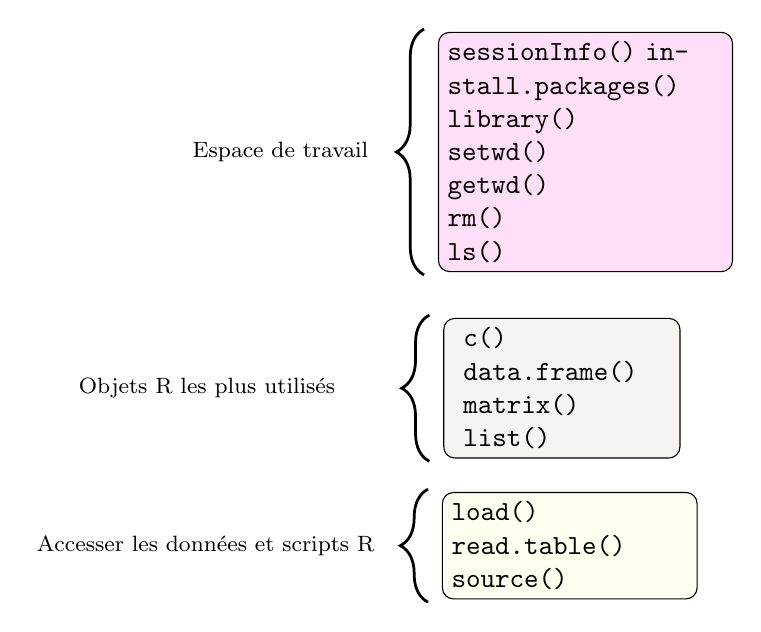
\begin{tikzpicture}
\node (expr) [startstop] {\code{sessionInfo()}
\code{install.packages()}
\code{library()}\textcolor{pinkish}{texxxx}
\code{setwd()}\textcolor{pinkish}{teccc}
\code{getwd()}\textcolor{pinkish}{teccc}
\code{rm()}\textcolor{pinkish}{tevvvvvvv}
\mbox{\code{ls()}\textcolor{pinkish}{tevvvvvvv}}  };
\node (fat) [startstop2, below of=expr, xshift=-.3cm, yshift=-2.0cm] {\code{c()}
\code{data.frame()}
\code{matrix()}
\code{list()}};
\node (script) [startstop3, below of=fat, xshift=.1cm, yshift=-1.0cm] {\code{load()}
\code{read.table()}
\code{source()}};
\draw[decoration={brace,raise=5pt, amplitude=10pt},decorate,line width=1pt] 
  ([yshift=-1pt]expr.south west) -- ([yshift=1pt]expr.north west) node [black,midway,xshift=-2cm] 
{\footnotesize Espace de travail};
\draw[decoration={brace,raise=5pt,amplitude=10pt},decorate,line width=1pt] 
  ([yshift=-1pt]fat.south west) -- ([yshift=1pt]fat.north west) node [black,midway,xshift=-3cm] 
{\footnotesize Objets R les plus utilisés};
\draw[decoration={brace,raise=5pt,amplitude=10pt},decorate,line width=1pt] 
  ([yshift=-1pt]script.south west) -- ([yshift=1pt]script.north west) node [black,midway,xshift=-3cm] 
{\footnotesize Accesser les données et scripts R};
\end{tikzpicture}
%}
\end{frame}








\subsection{Les objets R}

\begin{frame}
 \begin{center}
  \Huge{\textcolor{red}{Les objets R}}
 \end{center}
\end{frame}


%\begin{frame}[<+->]{Les objets R}
%\begin{itemize}
%  \setlength\itemsep{2em}
%\item Tout dans le langage R est un objet:
%\begin{itemize}
%\item les variables contenant des données
%\item les fonctions, 
%\item les opérateurs, même le symbole représentant le nom d’un
%objet est lui-même un objet.
%\end{itemize}
%\end{itemize}
%\end{frame}




\begin{frame}{Les objets R}

\begin{itemize}
  \setlength\itemsep{2em}
\item Les structures de données peuvent être organisées par: 
\pause
\begin{enumerate}
\item leur dimension (1d, 2d, ou nd) 
\item si elles sont homogène ou hétérogène
\end{enumerate}
\pause \item Cela donne lieu à 5 types de données les plus souvent utilisées dans l'analyse des données:
\end{itemize}
\pause 
\ctable[caption={Les structures de données en R},label=tab:table1,pos=h!,doinside=\small]{ccccc}{\tnote{tous les éléments doivent être du même type}\tnote[b]{les éléments peuvent être de différent types}
}{
    																\FL
dimension	&  & homogène\tmark	    &	& hétérogène\tmark[b] \ML
1d & & Atomic vector & & List \NN
2d & & Matrix & & Data frame \NN
nd & & Array & &    \LL
}

\end{frame}


\begin{frame}[fragile]{Atomic vectors}

\begin{itemize}
  \setlength\itemsep{2em}
\item En R, à toutes fins pratiques, tout est un vecteur
\pause \item Il n'y a pas de notion de scalaire en R ; un scalaire est simplement un vecteur de longueur 1
\pause \item La fonction de base pour créer un vecteur est \code{c()}
\end{itemize}
\pause
\begin{knitrout}
\definecolor{shadecolor}{rgb}{1, 1, 1}\color{fgcolor}\begin{kframe}
\begin{rcode}\begin{alltt}
\hlkwd{c}\hlstd{(}\hlnum{1}\hlstd{,} \hlnum{2}\hlstd{,} \hlnum{5}\hlstd{)}
\end{alltt}
\begin{verbatim}
## [1] 1 2 5
\end{verbatim}
\end{rcode}\end{kframe}
\end{knitrout}

\end{frame}




\begin{frame}[fragile]{Atomic vectors}

\begin{itemize}
  \setlength\itemsep{2em}
\item Les quatre types d'atomic vectors les plus utilisés: 
\begin{enumerate}
\item double (également appelé numeric)
\item integer
\item character
\item logical
\end{enumerate}
\end{itemize}
\pause
\begin{knitrout}
\definecolor{shadecolor}{rgb}{1, 1, 1}\color{fgcolor}\begin{kframe}
\begin{rcode}\begin{alltt}
\hlstd{num.var} \hlkwb{<-} \hlkwd{c}\hlstd{(}\hlnum{1}\hlstd{,} \hlnum{2.5}\hlstd{,} \hlnum{4.5}\hlstd{)} \hlcom{# numeric}
\hlstd{int.var} \hlkwb{<-} \hlkwd{c}\hlstd{(}\hlnum{1L}\hlstd{,} \hlnum{6L}\hlstd{,} \hlnum{10L}\hlstd{)} \hlcom{# integer}
\hlstd{chr.var} \hlkwb{<-} \hlkwd{c}\hlstd{(}\hlstr{"ceci sont"}\hlstd{,} \hlstr{"des characters"}\hlstd{)}
\hlstd{log.var} \hlkwb{<-} \hlkwd{c}\hlstd{(}\hlnum{TRUE}\hlstd{,} \hlnum{FALSE}\hlstd{, T, F)} \hlcom{# logical}
\end{alltt}
\end{rcode}\end{kframe}
\end{knitrout}

\end{frame}







\begin{frame}[fragile]{Test}

\begin{itemize}
  %\setlength\itemsep{1em}
\item \code{typeof()}: pour savoir quel type de vector
\item \code{is.character(), is.double(), is.integer(), is.logical(), is.atomic()}: pour vérifier si c'est un cas spécifique 
\end{itemize}
\pause
\begin{knitrout}\footnotesize
\definecolor{shadecolor}{rgb}{1, 1, 1}\color{fgcolor}\begin{kframe}
\begin{rcode}\begin{alltt}
\hlstd{int_var} \hlkwb{<-} \hlkwd{c}\hlstd{(}\hlnum{1L}\hlstd{,} \hlnum{6L}\hlstd{,} \hlnum{10L}\hlstd{)}
\hlkwd{typeof}\hlstd{(int_var)}
\end{alltt}
\begin{verbatim}
## [1] "integer"
\end{verbatim}
\begin{alltt}
\hlkwd{is.integer}\hlstd{(int_var)}
\end{alltt}
\begin{verbatim}
## [1] TRUE
\end{verbatim}
\begin{alltt}
\hlkwd{is.atomic}\hlstd{(int_var)}
\end{alltt}
\begin{verbatim}
## [1] TRUE
\end{verbatim}
\end{rcode}\end{kframe}
\end{knitrout}

\end{frame}



\begin{frame}[fragile]{Test}

\begin{knitrout}
\definecolor{shadecolor}{rgb}{1, 1, 1}\color{fgcolor}\begin{kframe}
\begin{rcode}\begin{alltt}
\hlstd{dbl_var} \hlkwb{<-} \hlkwd{c}\hlstd{(}\hlnum{1}\hlstd{,} \hlnum{2.5}\hlstd{,} \hlnum{4.5}\hlstd{)}
\hlkwd{typeof}\hlstd{(dbl_var)}
\end{alltt}
\begin{verbatim}
## [1] "double"
\end{verbatim}
\begin{alltt}
\hlkwd{is.double}\hlstd{(dbl_var)}
\end{alltt}
\begin{verbatim}
## [1] TRUE
\end{verbatim}
\begin{alltt}
\hlkwd{is.atomic}\hlstd{(dbl_var)}
\end{alltt}
\begin{verbatim}
## [1] TRUE
\end{verbatim}
\end{rcode}\end{kframe}
\end{knitrout}

\end{frame}



\begin{frame}[fragile]{Coercion}

\begin{itemize}
  \setlength\itemsep{1em}
\item Tous les éléments d'un atomic vector doivent être du même type
\pause \item Lorsque vous essayez de combiner différents types, ils seront convertis du type le plus flexible
\pause \item Types de moins à plus flexible sont:
\begin{enumerate}
\item logical 
\item integer 
\item double 
\item character
\end{enumerate}
\end{itemize}
\begin{knitrout}
\definecolor{shadecolor}{rgb}{1, 1, 1}\color{fgcolor}\begin{kframe}
\begin{rcode}\begin{alltt}
\hlcom{# combiner un character et integer donne un character}
\hlkwd{str}\hlstd{(}\hlkwd{c}\hlstd{(}\hlstr{"a"}\hlstd{,} \hlnum{1}\hlstd{))}
\end{alltt}
\begin{verbatim}
##  chr [1:2] "a" "1"
\end{verbatim}
\end{rcode}\end{kframe}
\end{knitrout}
\end{frame}



\begin{frame}[fragile]{Coercion}
\begin{itemize}
\item La plusplart des opérations mathématiques vont convertir un atomic vector à un double ou integer
\end{itemize}
\begin{knitrout}\footnotesize
\definecolor{shadecolor}{rgb}{1, 1, 1}\color{fgcolor}\begin{kframe}
\begin{rcode}\begin{alltt}
\hlstd{x} \hlkwb{<-} \hlkwd{c}\hlstd{(}\hlnum{FALSE}\hlstd{,} \hlnum{FALSE}\hlstd{,} \hlnum{TRUE}\hlstd{)}
\hlkwd{as.numeric}\hlstd{(x)}
\end{alltt}
\begin{verbatim}
## [1] 0 0 1
\end{verbatim}
\begin{alltt}
\hlcom{# Nombre total de TRUE}
\hlkwd{sum}\hlstd{(x)}
\end{alltt}
\begin{verbatim}
## [1] 1
\end{verbatim}
\begin{alltt}
\hlcom{# La proportion de TRUE}
\hlkwd{mean}\hlstd{(x)}
\end{alltt}
\begin{verbatim}
## [1] 0.33
\end{verbatim}
\end{rcode}\end{kframe}
\end{knitrout}
\end{frame}


\begin{frame}{Les objets R}

\ctable[caption={Les structures de données en R},label=tab:table1,pos=h!,doinside=\small]{ccccc}{\tnote{tous les éléments doivent être du même type}\tnote[b]{les éléments peuvent être de différent types}
}{
    																\FL
dimension	&  & homogène\tmark	    &	& hétérogène\tmark[b] \ML
1d & & Atomic vector & & \textcolor{red}{\textbf{List}} \NN
2d & & Matrix & & Data frame \NN
nd & & Array & &    \LL
}

\end{frame}



\begin{frame}[fragile]{List}

\begin{itemize}
  %\setlength\itemsep{2em}
\item Les lists sont différent des atomic vectors parce que leurs éléments peuvent \^{e}tre de tout type
\item La fonction pour créer un list est \code{list()}
\end{itemize}
\pause
\begin{knitrout}\footnotesize
\definecolor{shadecolor}{rgb}{1, 1, 1}\color{fgcolor}\begin{kframe}
\begin{rcode}\begin{alltt}
\hlstd{(x} \hlkwb{<-} \hlkwd{list}\hlstd{(}\hlnum{1}\hlopt{:}\hlnum{3}\hlstd{,} \hlstr{"a"}\hlstd{,} \hlkwd{c}\hlstd{(}\hlnum{TRUE}\hlstd{,} \hlnum{FALSE}\hlstd{,} \hlnum{TRUE}\hlstd{),} \hlkwd{c}\hlstd{(}\hlnum{2.3}\hlstd{,} \hlnum{5.9}\hlstd{)))}
\end{alltt}
\begin{verbatim}
## [[1]]
## [1] 1 2 3
## 
## [[2]]
## [1] "a"
## 
## [[3]]
## [1]  TRUE FALSE  TRUE
## 
## [[4]]
## [1] 2.3 5.9
\end{verbatim}
\end{rcode}\end{kframe}
\end{knitrout}

\end{frame}




\begin{frame}[fragile]{Attributs}

\begin{itemize}
  %\setlength\itemsep{2em}
\item Les attributs d'un objet sont des éléments d'information additionnels liés à cet objet
\item Pour chaque attribut, il existe une fonction du même nom servant à extraire l'attribut correspondant d’un objet
\end{itemize}

\ctable[caption={Attributs les plus usuels d'un objet},label=tab:table1,pos=h!,doinside=\small]{ccccc}{
}{
    																\FL
Attribut	&  & Utilisation \ML
class & & affecte le comportement d’un objet \\
dim & & dimensions des matrices et tableaux \\
dimnames & & étiquettes des dimensions des matrices et tableaux \\
names & & étiquettes des éléments d’un objet\LL
}



\end{frame}





\section{3. Graphiques}

\setbeamercolor{normal text}{fg=gray,bg=black}
\begin{frame}[plain]
\hspace*{-1.0cm}\parbox[t]{\textwidth}{
 \begin{center}
  \Huge{\textcolor{white}{3. Graphiques}}
 \end{center}
 }
\end{frame}

\setbeamercolor{normal text}{fg=gray,bg=white}
\subsection{Les objets R}

\begin{frame}
 \begin{center}
  \Huge{\textcolor{red}{Les objets R}}
 \end{center}
\end{frame}




\section{4. Statistiques}

\setbeamercolor{normal text}{fg=gray,bg=black}
\begin{frame}[plain]
\hspace*{-1.0cm}\parbox[t]{\textwidth}{
 \begin{center}
  \Huge{\textcolor{white}{4. Statistiques}}
 \end{center}
 }
\end{frame}

\setbeamercolor{normal text}{fg=gray,bg=white}
\subsection{Les objets R}

\begin{frame}
 \begin{center}
  \Huge{\textcolor{red}{Les objets R}}
 \end{center}
\end{frame}



\section{5. Cr\'{e}er des rapports reproductibles}

\setbeamercolor{normal text}{fg=gray,bg=black}
\begin{frame}[plain]
\hspace*{-1.0cm}\parbox[t]{\textwidth}{
 \begin{center}
  \Huge{\textcolor{white}{5. Cr\'{e}er des rapports}}
 \end{center}
 }
\end{frame}

\setbeamercolor{normal text}{fg=gray,bg=white}
\subsection{Les objets R}

\begin{frame}
 \begin{center}
  \Huge{\textcolor{red}{Les objets R}}
 \end{center}
\end{frame}
















\end{document}
